\chapter{Technical details of Embree and the target application ART}

Some introduction stuff.¸ \todo{do}

\section{A brief introduction to ART}
\label{chap:art}

The Advanced Rendering Toolkit (ART), serves as the environment in which Embree shall be integrated into. Therefore, this chapter provides a brief introduction to ART to familiarize the reader with its core mechanics. Apart from a short description of the general workflow of ART, only its aspects that are relevant for the integration of Embree are considered in this chapter. For a more detailed description of ART and the scene description language, we would like to refer the reader to the ART Handbook \cite{arthandbook} and the ARM File Reference Manual \cite{artreferencemanual}.\footnote{It should be mentioned here that at the time of writing this thesis, both documents are still work in progress, and therefore incomplete. However, they will be expanded in the future.}

The latest version of ART at the time of writing this thesis is Version 2.0.3.


\subsection{Purpose and features}

As indicated in the introduction, ART considers its target audience computer graphics researchers who are interested in the field of predictive rendering. Predictive rendering is a branch of the computer graphics field that is dedicated to the research of light transport simulation, with which one can accurately predict the appearance of tan object or a virtual scene under different viewing conditions (compare \cite{wilkie2009predictive}.) \todo{use Alban's example} While the purpose of "conventional rendering" (to which we count the rendering procedures encountered in Chapter \ref{chap:fundamentals}) lies in the creation of "believable" imagery to create a certain impression to an observer, predictive rendering is concerned with the synthesis of radiometrically correct images, which serve as matters of conducting actual research as opposed to communicating a visual impression on an observer.

ART offers a variety of important features for predictive rendering that are currently non-standard in other "mainstream" rendering systems, such as polarization visualization support, the physically plausible handling of fluorescent materials \cite{mojzik2018handling}, and the enabling of spectral rendering. For the later, ART implements the "Hero wavelength spectral sampling" technique \cite{wilkie2014hero} and utilizes its own spectral image file format. Additionally, various research projects belonging to the "Sky Dome Appearance Project" are implemented in ART \cite{hosek2012analytic, hovsek2013adding, wilkie2013predicting}.


\subsection{Overview}
ART	is composed of a number of UNIX-like-command line applications (therefore the name Advanced Rendering \emph{Toolkit}). The applications are written in \texttt{C} and \texttt{Objective-C}. 

In the following, we provide an overview over the individual applications contained in the toolkit:
\begin{description}
	% \setlength\itemsep{0.05em}
	\item[\emph{artist}] \hfil \\ This is the actual command-line application renderer, taking an ARM scene file as input and storing the raw information gathered by path tracing process in an intermediate file described in a proprietary file format. This file is not an image file one can display in an image viewing application.
	\item[\emph{tonemap}] \hfil \\ This tool can be used for tone-mapping the (possibly spectral) information stored in the file being created by \texttt{artist} in order to obtain viewable results.
	\item[\emph{bugblatter}] \hfil \\ This application creates difference images of two provided, same-sized images. These difference images can be useful when debugging computer graphics applications.
	\item[\emph{polvis}] \hfil \\ Since ART supports rendering polarization effects by storing the amount of polarized light per pixel in each pixel of a spectral image, these polarization effects can be visualized by the use of this tool.
	\item[\emph{impresario}] \hfil \\ With this application it is possible to store and display intermediate rendering results from currently running rendering jobs. This application is similar to a software daemon.
\end{description}

For our integration of Embree, the only relevant application is \texttt{artist}. 

In order to successfully render an image with \texttt{artist}, in the ARM scene file, one has to at least provide a virtual camera, the scene geometry, and an action sequence. An action sequence is a user defined procedure, telling ART how to render the provided scene. Functionality of other applications like \texttt{tonemap} or \texttt{polvis} can be included in an action sequence.
In order to execute the individual steps  defined by an action sequence (which are referred to as \emph{actions}), ART makes use of a single stack data structure. During the execution of one such action, one or multiple data objects are taken off the stack, manipulated according to the action in question, and placed back on the stack. One example of such an action would be the creation of axis aligned bounding boxes for each object present in the scene. Here, the scene graph object is popped from the stack, bounding boxed are calculated for each geometry, then these boxes are inserted into the scene graph. Further bounding boxes, enclosing these for the geometries are calculated and inserted into the scene graph, too. Finally, the manipulated scene graph is pushed back to the stack.

Another noteworthy detail to mention is the ability of ART to utilize multiple available processor cores to perform a rendering job. By default, ART determines the number of available cores before the path tracing, however, a number of a desired amount of cores to perform the rendering job can be provided by invoking

\begin{Verbatim}
artist foo.arm -j<n>
\end{Verbatim}

where \texttt{<n>} is the number of preferable cores.

To achieve lock free parallelism between the individual threads, the scene graph is copied and one such copy is assigned to each thread. 
 

\subsection{Scene graph infrastructure}
Some popular rendering systems (among them Mitsuba 2 and pbrt) describe a virtual scene in the following way: A virtual scene, abstracted by a \texttt{Scene} class object, obtains a collection of geometric shapes. These shapes are represented by a \texttt{Shape} base class, which offers functions for calculating its bounding box and performing intersection tests with a given ray. Various shape types can be represented as a child classes of this \texttt{Shape} class. This is an ideal design for Embree since these shapes can be initialized as User Defined Geometries. Once Embree finds an intersection with a bounding box of a particular shape, its representation in memory can be retrieved via the User pointer \todo{explain} and an instance function of the \texttt{Shape} class for ray-intersection testing can be called. 

\begin{figure}
	\centering
	
	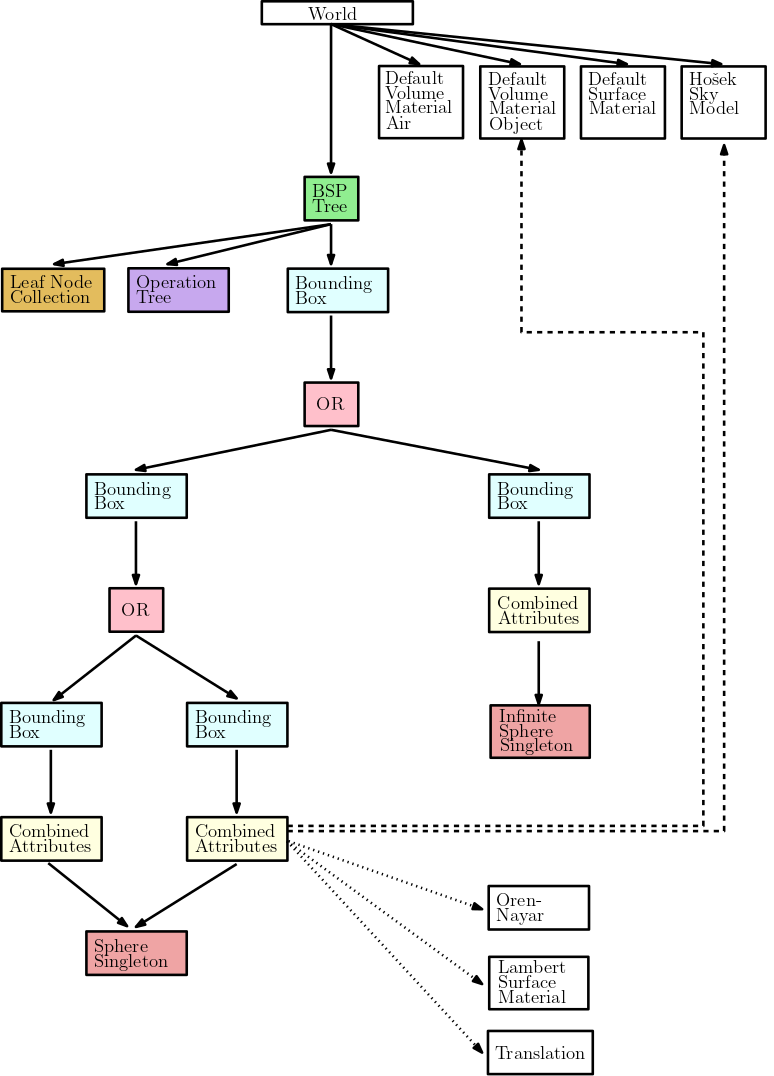
\includegraphics[width=1\linewidth]{img/2 art/scene_graph.png}
	\caption{Scene graph used to render Figure \ref{fig:csg_or}. In this graph, bounding boxes have already been inserted and a KD tree was built over the scene.} 
	\label{fig:scene_graph}
\end{figure}

\begin{table}
  \centering
  {\footnotesize
    \begin{tabular}{m{3cm}m{8cm}}
      \toprule
      Scene graph node & Function  \\
      \midrule
      
\includegraphics[scale=0.5]{img/2 art/shape_node.png} & This node belongs
                                                              to the category of
                                                              "shape nodes" that
                                                              are associated
                                                              with the
                                                              representation of
                                                              a geometry by
                                                              ART. Nodes of this
                                                              type are always
                                                              leafs.\\
      \midrule
      
\includegraphics[scale=0.5]{img/2 art/comb_attr_node.png} & This node is
      \\
      \midrule
    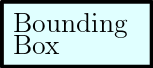
\includegraphics[scale=0.5]{img/2 art/bounding_box.png} & This node
                                                                       represents
                                                                       a
                                                                       bounding
                                                                       box,
                                                                       enclosing
                                                                       the
                                                                       components
                                                                       of the
                                                                       sub tree
                                                                       rooted at
                                                                       the
                                                                       node. \\
      \midrule
     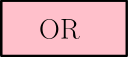
\includegraphics[scale=0.5]{img/2 art/or.png} & Nodes with two
                                                              children,
                                                              representing the
                                                              primitives to
                                                              which this CSG
                                                              operation is
                                                              applied to (in
                                                              this example, it
                                                              the two nodes are
                                                              representing the
                                                              union
                                                              operation). \\
      \midrule
     
\includegraphics[scale=0.5]{img/2 art/bsp_node.png} & Represents
                                                                    the KD tree
                                                                    that is
                                                                    build over
                                                                    the
                                                                    scene. Its
                                                                    children are
                                                                    the entire
                                                                    scene
                                                                    geometry, a
      \\
      \bottomrule
    \end{tabular}}
  \caption{Nodes in the scene graph displayed in Figure \ref{fig:scene_graph} and their functionality.}
  \label{tab:nodes}
\end{table}


The scene graph being utilized by ART diverges from this design. This section provides an overview over different nodes in the scene graph and their functionality on the basis of a provided example scene graph. This scene graph, which was used by ART to render the image displayed in Figure \ref{fig:csg_or}, is shown in Figure \ref{fig:scene_graph}. Table \ref{tab:nodes} displays its nodes and a brief description of their functionality and relation to other nodes. However, we will only list nodes for which the comprehension of their functionality is important to follow the implementation description in the next chapter.
On particularity of the scene graph is that it can be utilized by every application mentioned in the previous section, with the exception of \emph{impresario}.

\subsection{Ray Tracing with ART}
\label{sec:art_raytracing}
The functionality redarding ray tracing in ART is abstracted in the \texttt{ArnRayCaster} class. This class is inherited from the \texttt{ArnGraphTraversal} class. 

\todo{talk this over with Alban}

\todo{talk about org scene graph rendering}

\begin{figure}[!tbp]
	\centering
	\subfloat[Image rendered by traversing the KD Tree.]{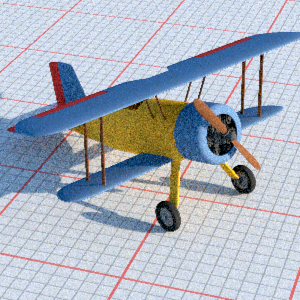
\includegraphics[width=.4\textwidth]{img/2 art/plane.png}}
	\hfill
	\subfloat[Image renderd by traversing the original scene graph.]{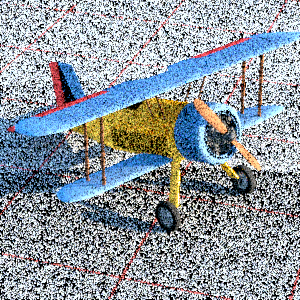
\includegraphics[width=.4\textwidth]{img/2 art/planeArtifacts.png}}
	\caption{Comparison of rendered images by traversing ART's internal KD tree and traversing the original scene graph.}
	\label{fig:org_scenegraph}
\end{figure}

\todo{talk about intersection list}

\section{Ray Tracing with Embree}
\label{sec:embree_raytracing}
Embree follows a device concept, allowing for the use of the Embree API by different components of the image synthesis application without interfering each other. An \texttt{RTCDevice} can be created with the function \texttt{rtcNewDevice} and released via the function \texttt{rtcReleaseDevice}. Such device types are used by Embree to create further components, such as virtual scenes which serve as the container for various scene geometry. A scene in Embree, represented by the data type \texttt{RTCScene}, can be created via the function \texttt{rtcNewScene}, to which the \texttt{RTCDevice} is passed to as an argument, and released via the function \texttt{rtcReleaseScene}. Different geometries can be attached or detached by the functions \texttt{rtcAttachGeometry}, which will furthermore assign a unique ID to the geometry, and \texttt{rtcDetachGeometry}. Once an \texttt{RTCGeometry} is attached to the \texttt{RTCScene}, it can be released via the call of the function \texttt{rtcReleaseGeometry}.
After the attachment of the complete scene geometry, the scene can be committed by calling the function \texttt{rtcCommitScene} in order to trigger the creation of Embree's internal acceleration structures. After the invocation of this function, the individual geometries cannot be edited or manipulated.

Geometries in Embree are represented by a \texttt{RTCGeometry} data type. These types can be created with the function \texttt{rtcNewGeometry} which takes the \texttt{RTCDevice} and an enum specifying the geometry type (e.g. triangle, quad, user defined geometry) as input parameters. In case the geometry being a triangle, quadrangle or a type of curve, so-called \emph{geometry buffers} can be created and linked to the \texttt{RTCGeometry} by invoking the function \texttt{rtcSetNewGeometryBuffer}. These buffers will store information such as vertices, indices and surface normals of the geometry.  

In order to initialize a user defined geometry, one has to provide a function for calculating the bounding box for the geometry, a function for intersection testing and another function for occlusion testings. These functions are passed to Embree as callback functions. Furthermore, the number of geometric primitives, which together compose the geometry, has to be set, and a so-called \emph{User data pointer} associated with the geometry. A user data pointer points to the representation of the geometry by the rendering application in memory. This user data pointer can be associated with geometry types other than user defined geometry.
In the interior of the callback function for calculating the intersection with the user defined geometry, the original representation of the geometry can be easily retrieved via this pointer. The passing of the various callback functions to Embree is done via invocation of the functions \texttt{rtcSetGeometryUserPrimitiveCount}, \texttt{rtcSetGeometryUserData}, \texttt{rtcSetGeometryBoundsFunction}, \texttt{rtcSetGeometryIntersectFunction}, \newline and \texttt{rtcSetGeometryOccludedFunction}.

Once the \texttt{RTCDevice} and the \texttt{RTCScene} are set up, the scene geometry is attached to the \texttt{RTCScene}, and the internal acceleration data structures have been built, nothing stands in the way of performing the actual ray tracing with Embree. 

In the following example, only ray tracing with single rays as opposed to packet ray tracing is considered. We will furthermore not consider instancing, due to the reason that this feature does not find use in the work of this thesis.

In order to ray trace a virtual scene, a per ray query intersection context, \texttt{RTCIntersectContext}, has to be set up via the function \texttt{rtcInitIntersectContext}. This structure is used for the configuration of intersection flags, among other things. 
Subsequently, a \texttt{RTCRayHit} struct is declared. This struct is composed of an \texttt{RTCRay} struct, abstracting the ray that is used by Embree to preform the intersection testing, and an \texttt{RTCHit} struct, in which information concerning the intersection point, such as the surface normal, the barycentric UV coordinates of the point, and the geometry ID associated with the intersected geometry are stored.
The \texttt{RTCRay} struct stores the ray orientation and direction, so-called \texttt{tnear} and \texttt{tfar} values, indicating the boundaries of a range of possible hit distances, and other information such as an id for the ray, a ray mask and a \texttt{time} value useful when motion blur is desired.
When the target ray tracing application is generating a ray, the values of the \texttt{RTCRay} struct are updated with the ray orientation and direction. The \texttt{tnear} value is usually set to zero and the \texttt{tfar} value is set to infinity. The geometry ID of the \texttt{RTCHit} struct is initialized with the macro \texttt{RTC\_INVALID\_GEOMETRY\_ID}.

After the \texttt{RTCIntersectContext} and the \texttt{RTCRayHit} structs have been successfully initialized and updated, the ray-primitive intersection testing is performed via invocation of the function \texttt{rtcIntersect1} to which the \texttt{RTCScene}, a reference to both the \texttt{RTCIntersectContext} and the \texttt{RTCRayHit} are passed as arguments. In case of a found intersection, this function will update the \texttt{tfar} value of the \texttt{RTCRay} with the closest hit distance and the geometry ID of the \texttt{RTCHit} with the geometry ID associated to the intersected geometry.

In case of performing intersection testing between a user defined geometry and a ray, these values have to be updated manually inside the intersection function that was passed to Embree as a callback function.

When the intersecting testing procedure has finished, the geometry ID of the \texttt{RTCHit} will give insight on whether an intersection was found or not. If the value of this variable remains \texttt{RTC\_INVALID\_GEOMETRY\_ID}, one can conclude that no intersection was found. Otherwise, an intersection was found and the \texttt{RTCRay} and \texttt{RTCHit} components of the \texttt{RTCRayHit} will provide the hit distance, the coordinates of the surface normal at the intersection point and the UV coordinates of the intersection point.

